\documentclass{article}

% Language setting
% Replace `english' with e.g. `spanish' to change the document language
\usepackage[danish]{babel}
% Set page size and margins
% Replace `letterpaper' with `a4paper' for UK/EU standard size
\usepackage[a4paper,top=2cm,bottom=2cm,left=3cm,right=3cm,marginparwidth=1.75cm]{geometry}

% Useful packages
\usepackage{amsmath}
\usepackage{graphicx}
\usepackage[colorlinks=true, allcolors=blue]{hyperref}
\usepackage{array}
\usepackage{subfig}
\usepackage{subfigure}
\usepackage{titlesec}


\title{CDIO delopgave 0}
\author{Jakob Agergaard}

\linespread{1.25}
\begin{document}
\titlespacing{\section}
    {0pt}{2em}{1em}




\begin{titlepage}
\begin{center}

    
\includegraphics[width=0.25\textwidth]{Billeder/DTULogo.png} \\
    \vspace{0.5cm}
    \Large
    \textbf{02314\hspace{1cm}62531\hspace{1cm}62532} \\
    Indledende programmering, Udviklingsmetoder til IT-systemer og Versionsstyring og testmetoder
    \vspace{0.4cm}
    \hrule
    
    \vspace*{0.5cm}
    \huge
    \textbf{CDIO delopgave 0}\\
    \LARGE
    Gruppe 17
    \vspace{0.5cm}
    \hrule
    \vspace{0.2cm}

    \large
    \begin{tabular}{m{10em} m{8em} m{8em} m{10em}}
    Jakob Skov Agergaard\vfill s224570 & 
\includegraphics[width=0.2\textwidth]{Billeder/JakobFoto.png} & 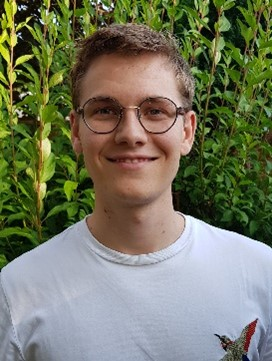
\includegraphics[width=0.2\textwidth]{Billeder/PhilipFoto.jpg} & Philip Muff Førrisdahl\vfill s224566 \\
    Mads Fogelberg Hansen\vfill s224563 & 
\includegraphics[width=0.2\textwidth]{Billeder/FotoMads.jpg} & 
\includegraphics[width=0.2\textwidth]{Billeder/EsbenFoto.png} & Esben Skovmand Elnegaard \vfill s224555  \\
    Jarl Boyd Roest\vfill s224556 & 
\includegraphics[width=0.2\textwidth]{Billeder/JarlFoto.png}
    \end{tabular}

    \vfill
    
    
    \vspace{1cm}
    \LARGE
    18. september 2022

    \vspace{1cm}
    
\end{center}
\end{titlepage}


\normalsize
\begin{abstract}

Ud fra kundens vision er der blevet udarbejdet en rapport, som indeholder et terningespil  som ønsket. Ved hjælp af krav og kundens vision, er der blevet fremstillet en analyse i form af en use case beskrivelse. Use case beskrivelsen beskriver de funktioner, som programmet skal indeholde for at kunne køre efter kundens vision og krav. Derudover er der lavet en test, der kontrollerer at en spillers pointbalance ikke kan blive negativ. Der er til slut blevet lavet en konklusion, som konkludere at der er blevet fremstillet et program, som opfylder kundens krav og vision.
\end{abstract}
\break

\tableofcontents

\break

\section{Timeregnskab}
\begin {itemize}
\item Arbejdsdag 1: 2 timer
\item Arbejdsdag 2: 2,5 timer 
\item Arbejdsdag 3: 2 timer 
\item Arbejdsdag 4: 1 time
\item Arbejdsdag 5: 2 timer
\end {itemize}

\section{Indledning}

I denne rapport, giver vi et indblik i vores udviklingsproces af spillet terningspil V2.  Vi har udviklet spillet, på baggrund af kundens vision, med vejledning af projektlederne for at præcisere krav. Arbejdsprocessen har forsøgt a følge Rational Unified Process. Dermed har arbejdet foregået i små iterationer med evaluering mellem. 

\section{Projekt-planlægning}
\begin {itemize}
\item [\textbf{Begyndelsen:}]På dag et, sørgede vi for at stille projektlederen relevante spørgsmål for at opnå en kravsspecifikation der var detaljeret og som levede op til forventninger fra alle parter.\\
Her udarbejdede vi også vores korte use case.
\item [\textbf{22-10-2022:}] Vi mødtes på discord for at få et overblik over hvor langt vi var i processen, samt for at arbejde videre på projektet. Her blev der startet på system-sekvensdiagram

 \item [\textbf{Uge 1:}]

\end {itemize}

\section{Krav \& Analyse}
\subsection{Spørgsmål til og svar fra projektlederen}

\begin{itemize}
    \item [Q:] Hvad vil det sige at "Det skal være let at skifte til andre terninger"?
            \subitem A: Man skal let kunne ændre i klassen, så der kan skriftes til et andet antal sider.
    \item [Q:] Hvad vil det sige at "Spillet skal let kunne oversættes til andre sprog."?
            \subitem A: En oversætter skal kunne tilgå alt tekst, uden at skulle rode for meget rundt i koden.
    \item [Q:] Er det nødvendigt at spillerne har andre navne end “spiller 1 og 2”
            \subitem A: Det er op til os som udviklere.
    \item [Q:] Hvad vil det sige at der skal "udskrives en tekst omhandlende det aktuelle felt"? Skal vi selv finde på en tekst?
            \subitem A: Når der landes på et felt skal der udskrives en tekst, som vi selv kan finde på. Den skal som minimum give information om hvilket felt det drejer sig om.
    \item [Q:] Kan man gå i negativ pengebeholdning?
            \subitem A: Nej, det kan man ikke. 
\end{itemize}
\subsection{Kravsliste}
\begin{itemize}
    \item Skal kunne spilles på DTU's maskiner i databarer
    \item To terninger
    \item Hver spiller har en pengebeholdning, der starter på 1000
    \item Spil indeholder felter med numrene fra 2-12
    \item Felter påvirker spillernes pengebeholdning (se bilag 1 for værdiliste)
    \item Pengebeholdninger skal kunne benyttes i andre spil
    \item Udskrivning af tekst der matcher feltet
    \item Skal kunne oversættes til andre sprog (have alle prints i samme klasse)
    \item Antallet af sider på terningerne skal kunne ændres af kunden (ikke brugeren)
   
    
\end{itemize}

\subsection{Use case beskrivelse }
\textbf{Scope:} Spil terningespil\\
\textbf{Level:} Spillere\\
\textbf{Primary actor:} Spiller 1 og spiller 2\\
\textbf{Stakeholders and interests:}\\
- Spillere: Vil have et underholdene spil der virker hurtigt og korrekt.\\
- Projektlederne: Vil gerne kunne tilfredsstille kundens ønsker.\\
- kunden: Vil gerne have et spil, der kan spilles på DTU's databarer.\\
\textbf{Preconditions:} Der er styresystemet "Windows" på maskinerne og den nyeste version af Java. Desuden besidder brugeren over 8. klasse pc færdighed, er op til 80 år gamle og har et almindeligt helbred.\\
\textbf{Succes Guarantee:} Spillet afsluttes og angiver en vinder.\footnote{Gruppe 17 CDIO 1}\\

\textbf{Main Success Scenario}
\begin{enumerate}
\itemsep-0.5em
    \item Første spiller slår med terningerne
    \item Systemet lægger øjnene på terningerne sammen
    \item Første spillers brik bliver nu rykket det antal felter som terningernes øjne viser
    \item System fortæller spilleren hvilket felt de er landet på og udskriver en kort beskrivelse af feltet, herunder hvor mange point man får på det givne felt.
    \item Pointene bliver tilføjet/fratrukket spillerens pengebeholdning
    \item Systemet skifter tur til næste spiller.\\
    \textit{Punkterne 1-6 bliver nu gentaget for næste spiller}
    \item Alle steps bliver nu gentaget indtil en spiller når en pengebeholdning på 3000 eller derover.
    \item Systemet udskriver en tekst der fortæller spillerne hvem der har vundet.
\end{enumerate}
\textbf{Extension (Alternate Succes Scenario): }
\begin{enumerate}
    \item [6.a] En spiller slår 10.
    \subitem 1. Punkterne 1-5 bliver gentaget for denne spiller (Ekstra tur)
\end{enumerate}

\textbf{Sub use cases (beskrevet på 'brief format'):}
\begin{itemize}
    \item Ryk brik
    \item Slå terninger
    \item Få point
    \item Mist point
    \item Skift tur
\end{itemize}

\textbf{Use case skrevet på 'fully dressed' format:}\\
Første spiller trykker på enter for at starte spillet, og slår dermed også med begge terninger. Systemet udskriver dernæst hvilket felt spilleren er landet på, samt en kort beskrivelse af hvilken indflydelse feltet har på spillerens pengebeholdning.\\
Det er nu den anden spillers tur, og spilleren slår også med begge terninger. Systemet udskriver, på samme måde som før, hvilket felt spilleren er landet på, samt en kort beskrivelse af hvilken indflydelse feltet har på spillerens pengebeholdning.\\
Disse steps gentages indtil en spiller har en pengebeholdning på 3000. Når dette sker udskriver systemet hvilken spiller der har vundet, og spillet er dermed slut.\\
\textbf{Use case diagram}
\begin{figure} [h]
    \centering
    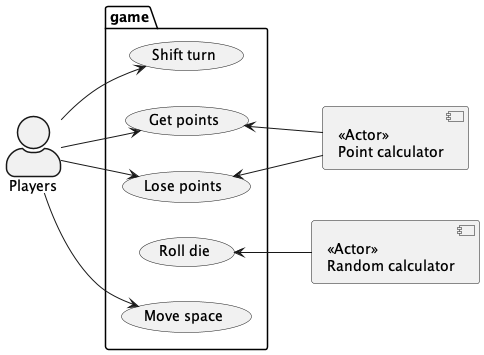
\includegraphics[width = 0.6\textwidth]{Billeder/UseCaseDiagram.png}
    \caption{Use case diagram}
\end{figure}
\section{Design}
Vi har med henblik på at få lavet det mest optimale og overskuelige kode, lavet 2 former for design diagrammer, der danner et simpelt overblik på vores program. Med use case realization, har vi holdt den råde tråd, og påmindede os selv på kravene programmet skal have. vi har startet ud med at lave et use case diagram (fig 2) og et klasse diagram (fig 4). Heraf har vi udviklet et design klasse diagram (fig. 3) , og et systemsekvens diagram(fig. 1), der hver i sær viser spillet på deres måde. Med denne fremgangsmåde fik vi hurtigt sat klasserne op, med de defineret objekter og metoder.
\\
\begin{figure} [h]
    \centering
    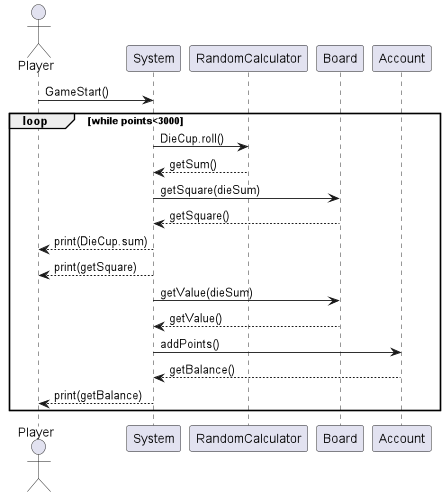
\includegraphics[width = 0.6\textwidth] {Billeder/System sequence diagram.png}
    \caption{System sequence diagram}
    \label{fig:Systemssekvensdiagram}
\end{figure}
\\

\\
\begin{figure} [h]
    \centering
    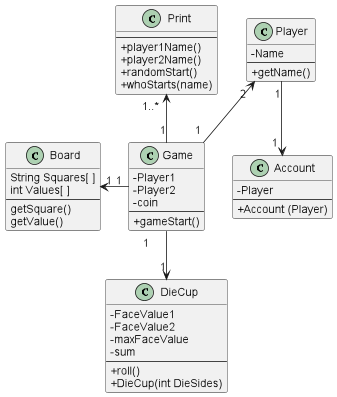
\includegraphics[width = 0.6\textwidth]{Billeder/Design class diagram.png}
    \caption{Design klasse diagram}
    \label{Design klasse diagram}
\end{figure}
\\
\begin{figure} [h]
    \centering
    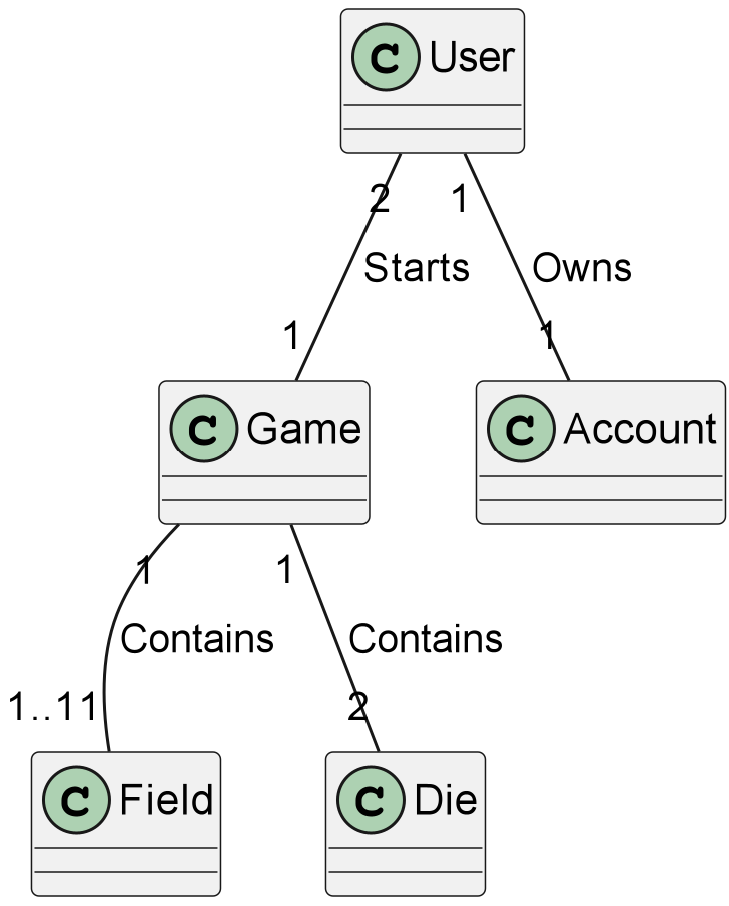
\includegraphics[width = 0.4\textwidth]{Billeder/Klassediagram.png}
    \caption{Klasse diagram}
    \label{Design klasse diagram}
\end{figure}
\\
\\
\\
\\
\section{Implementering}

Vi har valgt at ligge alle Strings, der bliver printet, i én klasse. Dette giver mulighed for nemt at ændre teksten til et andet sprog.\\


 
\section{Test}
Den primære årsag for at teste sit program er for at finde mulige fejl, men det kan også være for at kvalitetstjekke sit program eller forbedre det. Man bruger typisk iterativmetoden, og ikke vandfaldsmetoden, til at teste sit program, hvor man tester små bider af sit program løbende i programmerings processen. Dette gør at man løbende sikre sig at sit program fungere og lever op til kravene fra kunden. 
\\
\\Der er blevet efterspurgt en test af at en spillers balance ikke kan gå i negativ pengebeholdning.
\\Vores test er lavet på baggrund af af vores terningspil og tager derfor udgangspunkt der fra. Testen viser at pengebalancen ikke kan gå i negativ, som var det, der var efterspurgt.
\\
Man kan derudover teste terningerne, for at se om de slag man kaster fordeler sig rigtig efter normalfordelingen af to terninger. Dette vil foreksempel kunne vise at terningerne ikke er snyde terninger, hvor der kan være større sandsynlighed for at slå et højere tal med de to terninger. 

\section{Konfiguration}
Følgende beskrivelse udgør minimumskrav samt vejledning i hvordan kildekoden compiles, installeres og afvikles, samt hvordan koden importeres fra et git repository.\\
Som minimumskrav kræves det at styresystemet er af Windows version 10 eller mere. Computeren skal have java version 18 eller nyere.\\
 \textbf{Vejledning til kompilering, installering og afvikling:}
\begin{enumerate}
    \item Naviger til \href{https://github.com/Jakob-SA/CDIO-2}{Github repo for projektet}.
    \item Tryk på "code" drop-downmenuen og download ZIP (vær sikker på du befinder dig i "master"-branchen)
    \item Udpak filen
    \item Naviger til filen i en terminal og ind i mappen navngivet "src"
    \item Her skriver du følgende i terminalen: \textit{"javac Main.java"}. Dette kompilere programmet.
    \item Herefter skriver du: \textit{"java Main"} og programmet kører i kommandolinjen.
\end{enumerate}


\section{Konklusion}
Ud fra testen, design, implementering og analysen, der er blevet fremstillet et terningespil. I analyse delen  er der blevet analyserede på hvilke krav som kunden havde til sit spil, og hvordan man skulle tilgå dem. Derudover er der blevet lavet en Use Case beskrivelse, som beskriver hvilke funktioner der skal være tilstede i programmet, for at det fungere bedste muligt. Dernæst er programmet blevet illustrere i design diagrammer, som danner overblik over programmet, og gør det mere overskueligt og nemmere at kode selve programmet. 
Heraf kan konkluderes at der er blevet programmeret et terningespil Ud fra ovenstående tekst, kan det konkluderes at der er blevet fremstillet et terningespil med udgangspunkt i kundens krav og vision.

\section{Bilag}
\subsubsection{Bilag 1: Liste med værdier for felter}

    \centering
    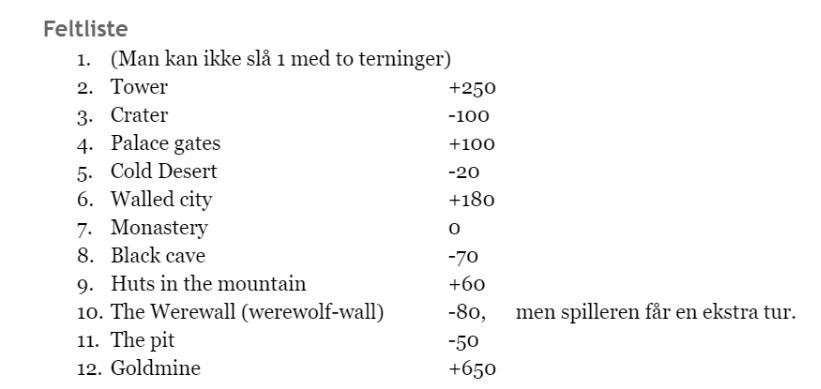
\includegraphics[scale=0.7]{Billeder/Bilag1Feltliste.png}
    \label{fig:Bilag1}

\subsubsection{Litteratur}
\begin{enumerate}
    \item Gruppe 17 - CDIO del 1 \\
    \href{https://github.com/Jakob-SA/CDIO-1}{https://github.com/Jakob-SA/CDIO-1}
\end{enumerate}

\subsubsection{Kode}
Koden produceret i projektet kan findes på følgende link: \href{https://github.com/Jakob-SA/CDIO-2}{https://github.com/Jakob-SA/CDIO-2}
\end{document}